\RequirePackage{fix-cm}
\documentclass[11pt,a4paper]{article}
\usepackage[utf8]{inputenc}
\usepackage[margin=2cm]{geometry}
\usepackage{amsmath,amssymb,mathtools}
\usepackage{booktabs,array,multirow}
\usepackage[most]{tcolorbox}
\usepackage{enumitem}
\setlist[itemize]{itemsep=1pt, topsep=2pt, label=$\bullet$}
\setlist[enumerate]{itemsep=1pt, topsep=2pt}
\usepackage{listings}
\usepackage{tikz}
\usetikzlibrary{arrows.meta,positioning,shapes.geometric,calc,fit}
\usepackage{pgfplots}
\pgfplotsset{compat=1.18}
% ---- matplotlib look for the plots drawn by LaTeX (no image files needed)
\definecolor{tabblue}{HTML}{1F77B4}\definecolor{taborange}{HTML}{FF7F0E}
\definecolor{tabgreen}{HTML}{2CA02C}\definecolor{tabred}{HTML}{D62728}
\pgfplotsset{mpl/.style={scale only axis, axis line style={black,line width=0.8pt},
  tick style={black,line width=0.8pt}, tick align=outside, xtick pos=bottom, ytick pos=left,
  major tick length=3.5pt, tick label style={font=\fontsize{10}{12}\selectfont\sffamily},
  legend cell align=left, legend style={draw=black!20, rounded corners=2pt, fill=white, fill opacity=0.8, text opacity=1},
  legend image code/.code={\draw[#1] (0pt,0pt) -- (22pt,0pt);}},
  mplgrid/.style={grid=major, major grid style={black!30, line width=0.8pt, dash pattern=on 2.96pt off 1.28pt}},
  mplmark/.style={legend image code/.code={\draw[mark repeat=2,mark phase=2,##1] plot coordinates {(0pt,0pt) (11pt,0pt) (22pt,0pt)};}}}
\tikzset{mpldash/.style={dash pattern=on 3.7pt off 1.6pt}, mpldot/.style={dash pattern=on 1pt off 1.65pt}}
% ---- flowcharts
\tikzset{
  fcbox/.style={rectangle, draw=DefBlue, line width=0.8pt, fill=DefBlue!4, align=flush center, font=\small, inner sep=3pt, minimum height=8mm},
  fcdec/.style={diamond, aspect=2.2, draw=LemRed, line width=0.8pt, fill=LemRed!4, align=flush center, font=\small, inner sep=2pt},
  fcterm/.style={rectangle, rounded corners=3mm, draw=AnsGreen, line width=0.8pt, fill=AnsGreen!8, align=flush center, font=\small, inner sep=3pt, minimum height=7mm},
  fcerr/.style={rectangle, rounded corners=3mm, draw=tabred, line width=0.8pt, fill=tabred!6, align=flush center, font=\small, inner sep=3pt, minimum height=7mm},
  fcplot/.style={rectangle, draw=taborange, line width=0.8pt, fill=taborange!7, align=flush center, font=\small, inner sep=3pt, minimum height=8mm},
  fcarr/.style={-{Stealth[length=2.2mm,width=1.8mm]}, line width=0.8pt},
  fcloop/.style={draw=CodeGray, line width=0.6pt, dashed, rounded corners=2mm, inner sep=2.5mm},
  fclab/.style={font=\footnotesize, text=CodeGray},
}
\usepackage{caption}
\usepackage{hyperref}
\hypersetup{colorlinks=true,linkcolor=black,citecolor=black,urlcolor=black,
  pdftitle={Financial Processes -- Homework 4: numerical Greeks},pdfauthor={Carlos Chipantiza}}
\usepackage{needspace}
\captionsetup{hypcap=false}
\frenchspacing
\emergencystretch=3em

\definecolor{DefBlue}{RGB}{16,64,120}
\definecolor{LemRed}{RGB}{170,30,40}
\definecolor{ThmPurple}{RGB}{95,40,130}
\definecolor{AnsGreen}{RGB}{20,120,70}
\definecolor{CodeGray}{RGB}{110,110,110}
\definecolor{FIX}{RGB}{20,120,70}

\newcounter{defn}\newcounter{lemn}\newcounter{thmn}\newcounter{corn}
\newtcolorbox{defbox}[1]{enhanced,colback=white,colframe=DefBlue,boxrule=0.8pt,arc=1mm,left=2mm,right=2mm,top=1.5mm,bottom=1.5mm,
  before upper={\refstepcounter{defn}\noindent\textbf{Definition \thedefn} (#1).\par\smallskip}}
\newtcolorbox{lembox}[1]{enhanced,colback=white,colframe=LemRed,boxrule=0.8pt,arc=1mm,left=2mm,right=2mm,top=1.5mm,bottom=1.5mm,
  before upper={\refstepcounter{lemn}\noindent\textbf{Lemma \thelemn} (#1).\par\smallskip}}
\newtcolorbox{corbox}[1]{enhanced,colback=white,colframe=LemRed,boxrule=0.8pt,arc=1mm,left=2mm,right=2mm,top=1.5mm,bottom=1.5mm,
  before upper={\refstepcounter{corn}\noindent\textbf{Corollary \thecorn} (#1).\par\smallskip}}
\newtcolorbox{thmbox}[1]{enhanced,colback=white,colframe=ThmPurple,boxrule=0.8pt,arc=1mm,left=2mm,right=2mm,top=1.5mm,bottom=1.5mm,
  before upper={\refstepcounter{thmn}\noindent\textbf{Theorem \thethmn} (#1).\par\smallskip}}
\newtcolorbox{stmbox}[1]{enhanced,colback=white,colframe=CodeGray,boxrule=0.8pt,arc=1mm,left=2mm,right=2mm,top=1.5mm,bottom=1.5mm,
  before upper={\noindent\textbf{Statement of the professor} (#1).\par\smallskip}}
\newtcolorbox{ansboxenv}{enhanced,colback=AnsGreen!6,colframe=AnsGreen,boxrule=0.8pt,arc=1mm,left=2mm,right=2mm,top=1.5mm,bottom=1.5mm}
\newcommand{\ansbox}[1]{\begin{ansboxenv}#1\end{ansboxenv}}
\newcommand{\subhead}[1]{\par\medskip\noindent{\large\bfseries #1}\par\smallskip\noindent\ignorespaces}
\newcommand{\step}[1]{\par\smallskip\noindent\textbf{#1}\enspace\ignorespaces}

% ---- code that can be copied from the PDF and pasted into Python:
% every space is a real character (an invisible glyph mapped to U+0020), no line
% numbers, no line breaks inside a line, straight quotes.
\input{glyphtounicode}
\pdfglyphtounicode{visiblespace}{0020}
\pdfgentounicode=1
\makeatletter
\def\lst@visiblespace{{\color{white}\char32}}
\makeatother
\lstdefinestyle{py}{language=Python,basicstyle=\ttfamily\footnotesize,keywordstyle=\color{DefBlue},
  commentstyle=\color{CodeGray},stringstyle=\color{black},showspaces=true,showstringspaces=false,
  frame=single,rulecolor=\color{CodeGray},numbers=none,
  breaklines=false,columns=fixed,basewidth=0.5em,keepspaces=true,tabsize=4,xleftmargin=0.4em,framexleftmargin=0.4em,
  captionpos=t,literate={\$}{{\char36}}1 {'}{{\char13}}1 {`}{{\char18}}1}
\lstdefinestyle{prof}{style=py,basicstyle=\ttfamily\fontsize{6.6}{7.8}\selectfont}
\lstdefinestyle{pysmall}{style=py,basicstyle=\ttfamily\fontsize{7.6}{9}\selectfont}
\lstdefinestyle{out}{basicstyle=\ttfamily\footnotesize,columns=fixed,basewidth=0.5em,showspaces=true,
  frame=leftline,framerule=1.2pt,rulecolor=\color{FIX},numbers=none,xleftmargin=0.8em,framexleftmargin=0.4em,
  breaklines=false,captionpos=t}
\captionsetup[lstlisting]{labelformat=empty,font={footnotesize,sf},justification=raggedright,singlelinecheck=false,skip=2pt}
\captionsetup[figure]{font=small}
\newcommand{\Et}{\tilde{E}}
\newcommand{\ul}{u_{\text{left}}}
\newcommand{\ur}{u_{\text{right}}}

\tikzset{
  inh/.style={-{Triangle[open,length=2.6mm,width=2.6mm]}, line width=0.8pt, CodeGray},
  usesa/.style={-{Stealth[length=2mm]}, line width=0.8pt, CodeGray},
  ghostb/.style={opacity=0.35, dashed},
  newb/.style={line width=1.6pt, label={[font=\tiny\bfseries, text=white, fill=taborange, inner sep=1.5pt]north east:NEW}},
  blab/.style={font=\scriptsize\itshape, fill=white, inner sep=1pt, align=center},
  lno/.style={font=\scriptsize\color{CodeGray}},
}
\newcommand{\Q}{\mathbb{Q}}
\newcommand{\ind}{\mathbf{1}}
\newcommand{\DF}{e^{-r\tau}}
\newcommand{\pos}[1]{\left(#1\right)^{+}}
\renewcommand{\subhead}[1]{\par\medskip\needspace{8\baselineskip}\noindent{\large\bfseries #1}\par\smallskip\noindent\ignorespaces}
\newcolumntype{L}[1]{>{\raggedright\arraybackslash}p{#1}}
\tikzset{
  updb/.style={line width=1.6pt, label={[anchor=south east, font=\tiny\bfseries, text=white, fill=taborange, inner sep=1.5pt]north east:UPDATED}},
  blk/.style={rectangle, draw=DefBlue, line width=0.8pt, fill=DefBlue!4, align=center, font=\footnotesize, inner sep=2.5pt},
  fccall/.style={rectangle, draw=taborange, line width=0.8pt, fill=taborange!7, align=flush center, font=\small, inner sep=3pt, minimum height=7mm},
}
% Block diagrams of the homework: which blocks exist after each piece of code.
% stage 1: enums (FDMethod, BumpType); 2: NEW VERSION of Pricer; 3: q1_fd_greeks_demo.py; 4: q1_bump_study.py.
\newcount\hwcur
\newcommand{\hwstage}[1]{%
  \ifnum\hwcur<#1\relax\tikzset{st#1/.style={ghostb},up#1/.style={},ast#1/.style={opacity=0.25},atx#1/.style={opacity=0.25}}%
  \else\ifnum\hwcur=#1\relax\tikzset{st#1/.style={newb},up#1/.style={updb},ast#1/.style={draw=taborange},atx#1/.style={text=taborange!80!black}}%
  \else\tikzset{st#1/.style={},up#1/.style={},ast#1/.style={},atx#1/.style={}}\fi\fi}
\newcommand{\stl}[2]{\ifnum\hwcur<#1\relax\textcolor{black!25}{#2}\else\ifnum\hwcur=#1\relax\textcolor{taborange!85!black}{\bfseries #2}\else #2\fi\fi}
\newcommand{\hwBlocksPic}[1]{%
\begin{tikzpicture}[every node/.style={font=\footnotesize}]
\hwcur=#1\relax
\hwstage{1}\hwstage{2}\hwstage{3}\hwstage{4}
% library of Lecture 6 (always there)
\node[blk, text width=3.1cm] (md) at (0,0) {\textbf{MarketData}, \textbf{VolGrid}\\ \texttt{mkt/*.csv} (Lecture 6)};
\node[blk, text width=3.1cm] (mm) at (0,-2.6) {\textbf{FlatVolModel}\\ $\sigma(K,T)$, \texttt{bump\_spot}\\ (sticky strike)};
\node[blk, text width=3.3cm, draw=taborange, fill=taborange!6] (ct) at (4.6,0) {\textbf{EuropeanContract}\\ CALL/PUT, $K$, $T$};
\node[blk, text width=3.3cm, draw=CodeGray, fill=CodeGray!6, st1] (en) at (9.2,0) {\textbf{enums.py}\\ \texttt{FDMethod}, \texttt{BumpType}};
\node[blk, text width=4.4cm, draw=AnsGreen, fill=AnsGreen!6, up2] (pr) at (6.2,-2.6) {\textbf{Pricer} (ABC)\\ \stl{2}{\texttt{fd\_method}, \texttt{bump\_type}}\\ \stl{2}{\texttt{absolute\_bump\_size}}\\ \stl{2}{bump size $h$; price at $S+kh$}\\ \stl{2}{\texttt{calc\_delta}, \texttt{calc\_gamma}: 6 schemes}};
\node[blk, text width=4.1cm, draw=AnsGreen, fill=AnsGreen!6] (ap) at (6.2,-5.4) {\textbf{EuropeanAnalyticPricer}\\ ANALYTIC $\Delta$, $\Gamma$ (Thm.~1)};
\node[blk, text width=3.2cm, draw=CodeGray, fill=CodeGray!6, st3] (dm) at (11.7,-2.6) {\textbf{q1\_fd\_greeks\_demo}\\ 6 combinations, checks};
\node[blk, text width=3.2cm, draw=CodeGray, fill=CodeGray!6, st4] (sd) at (11.7,-5.4) {\textbf{q1\_bump\_study}\\ 72 options, figures};
\draw[usesa] (mm) -- node[blab, right] {reads $S$, $r$, grid} (md);
\draw[usesa] (pr.west) -- node[blab, above] {deepcopy +} node[blab, below] {\texttt{bump\_spot}$(kh)$} (pr.west -| mm.east);
\draw[usesa] (ct.south) -- node[blab, right] {self.contract} (ct.south |- pr.north);
\draw[usesa, ast2] (pr.north east) -- node[blab, atx2, right=1pt] {labels} (en.south);
\draw[inh] (ap.north) -- (pr.south);
\draw[usesa, ast3] (dm) -- node[blab, atx3, above] {sets} (pr.east);
\draw[usesa, ast3] (dm.south west) -- node[blab, atx3, right=2pt] {greeks} (ap.north east);
\draw[usesa, ast4] (sd) -- node[blab, atx4, above] {72 pricers} (ap.east);
\end{tikzpicture}}
\newcommand{\hwBlocks}[2]{%
\begin{center}\begin{minipage}{\linewidth}\centering
\hwBlocksPic{#1}
\captionof{figure}{Blocks after #2. Bold with NEW: created by this code; UPDATED: changed by this code (orange lines); faded: still to come. Open triangle: inherits from; arrow: uses.}
\label{fig:blk#1}
\end{minipage}\end{center}}
\lstdefinestyle{outsmall}{style=out,basicstyle=\ttfamily\fontsize{6.9}{8.2}\selectfont}
\begin{document}
\noindent Name: Carlos Chipantiza \hfill Neptun code: EACN90\\
\noindent Financial Processes (BMETE95MM14), BME, Fall 2026 \hfill course id: 54932fw\\[2pt]
{\large\textbf{Homework 4 (Lecture 6): Numerical Greeks}}\\[2pt]
\noindent\rule{\textwidth}{0.4pt}

\noindent\textbf{Remark.} In this homework we are going to extend the numerical Greeks of Lecture 6: we add the three finite difference methods and the two bump types to the library, and then we measure their errors to choose the bump size. We use only results of the lectures; we state them in boxes with their cell and cite them by number. We need two short new facts (the one-sided second difference and the size of the error), which we deduce from the lecture's own construction and from calculus, with a reference. The code we show is an exact copy of the files, and every number is printed by it (files \texttt{*.out}). Files: the library of Lecture 6 (\texttt{contract.py}, \texttt{enums.py}, and \texttt{market\_data.py}, \texttt{model.py}, \texttt{pricer.py} of the \texttt{solution} folder) with the NEW CODE at the end of \texttt{enums.py} and the NEW VERSION of \texttt{Pricer} in \texttt{pricer.py}; the runs \texttt{q1\_fd\_greeks\_demo.py} and \texttt{q1\_bump\_study.py} (figures in \texttt{figures/}); the notebook \texttt{4\_HW\_EXE\_1} with the same code. The market data are the csv files of \texttt{QuantCourseBP/mkt}. Running example (Lecture 6, cell 22): ATM call on \texttt{BLUECHIP\_BANK}, $S=K=130.17$, $T=1$, \texttt{FlatVolModel} ($\sigma=0.38083$), $r=0.05$.

\subhead{1. The assignment.}
\begin{stmbox}{\texttt{notebook\_flatvol.ipynb}, cell 26}
\emph{Introduce two class variables in Pricer that store the finite difference method (forward, backward, central) to be used in numerical greek calculation, and whether the bump size is absolute or relative. Create two Enums to store the labels. Implement all combinations for delta and gamma calculation.\\
Compare greeks using the analytic and the finite difference approximation on a set of European options and visualize the numerical error. Compare absolute and relative bumping and suggest optimal bump sizes.} \textbf{(15 points)}
\end{stmbox}

% =====================================================================
\subhead{2. The problem.}
\begin{center}\small
\renewcommand{\arraystretch}{1.25}
\begin{tabular}{@{}L{0.2\textwidth}L{0.42\textwidth}L{0.32\textwidth}@{}}
\toprule
To build & What it must do & Lecture 6 pattern it follows\\
\midrule
two Enums & labels FORWARD, BACKWARD, CENTRAL and ABSOLUTE, RELATIVE & \texttt{GreekMethod} (\texttt{enums.py})\\
two class variables & choose the scheme of every numerical $\Delta$ and $\Gamma$ & \texttt{relative\_bump\_size} of \texttt{Pricer}\\
\texttt{calc\_delta}, \texttt{calc\_gamma} & $3$ methods $\times$ $2$ bump types (Definitions 1--2, Lemma 1) & central bump of \texttt{Pricer} (cell 25)\\
comparison & error of BUMP against ANALYTIC on a set of European options, plotted & task of cell 25\\
bump sizes & absolute against relative; the best $h$ & \texttt{relative\_bump\_size} $=0.01$\\
\bottomrule
\end{tabular}
\end{center}
\noindent The only mathematics we need is the six difference formulas and the size of their error (Section 3); everything else is code in the style of the lecture. Our plan is the following: first we state the results we are going to use, then we write the code and test it (Section 4), and finally we run it on a set of options to measure the errors and to choose the bumps (Section 5). We close with the conclusions (Section 6).

% =====================================================================
\subhead{3. Results used.}
\noindent\emph{From the lectures.} We start from what the lecture gives us: the difference formulas, the two kinds of bump, the analytic Greeks we compare with, and the model in which we bump.

\begin{defbox}{Finite differences; Lecture 6, cells 23--24}
Greeks are computed numerically ``using finite difference approximation (forward, backward, central)'' (cell 23). For a bump $h>0$:
\begin{equation}\label{eq:fd1}
\begin{aligned}
f'(x)&\approx\frac{f(x+h)-f(x)}{h} && \text{(forward)},\\
f'(x)&\approx\frac{f(x)-f(x-h)}{h} && \text{(backward)},\\
f'(x)&\approx\frac{f(x+h)-f(x-h)}{2h} && \text{(central)},
\end{aligned}
\end{equation}
and (cell 24) the central second difference, built as a central difference of central differences:
\begin{equation}\label{eq:fd2}
f''(x)\approx\frac{f'(x+\frac h2)-f'(x-\frac h2)}{h}\approx\frac{f(x+h)-2f(x)+f(x-h)}{h^2}.
\end{equation}
In the solution, \texttt{calc\_delta} and \texttt{calc\_gamma} use the central formulas and \texttt{calc\_theta} the forward one. For delta and gamma, $f(x)=V(S)$ is the fair value as a function of the spot.
\end{defbox}

\begin{defbox}{Absolute and relative bump; Lecture 6, cell 24 and \texttt{solution/pricer.py}}
The bump is \emph{absolute} when $h$ is a fixed number (the $\Delta$ of cell 24), and \emph{relative} when it is a fixed fraction of the spot,
\[
h=\varepsilon\,S,\qquad \varepsilon=\texttt{relative\_bump\_size}=0.01\ \text{in the lecture}.
\]
\end{defbox}

\begin{thmbox}{Black--Scholes delta and gamma; Lecture 3; Lecture 5, \texttt{pricer.py}}
With $d_1$ of the Black--Scholes formula and $\varphi=N'$, for a long European option
\begin{equation}\label{eq:bsgreeks}
\Delta_{\mathrm{call}}=N(d_1),\qquad \Delta_{\mathrm{put}}=-N(-d_1),\qquad \Gamma=\frac{\varphi(d_1)}{S\sigma\sqrt T}.
\end{equation}
In the library: \texttt{calc\_delta}, \texttt{calc\_gamma} with \texttt{GreekMethod.ANALYTIC}.
\end{thmbox}

\begin{defbox}{Flat volatility model, sticky strike; Lecture 6, cell 18 and \texttt{solution/model.py}}
For a contract $(K,T)$ the model reads $\sigma(K,T)$ on the surface and uses it in Black--Scholes. A bumped spot does not change $K$, so the bumped model reads the same $\sigma(K,T)$ (comment of \texttt{FlatVolModel.get\_vol}).
\end{defbox}
\noindent Because the FlatVol model keeps $\sigma(K,T)$ fixed when we bump the spot, the bumped prices $V(S\pm h)$ are Black--Scholes prices with the same $\sigma$. Therefore Theorem~1 gives exactly the derivative that the differences of Definition~1 approximate, and the difference BUMP $-$ ANALYTIC that we measure is the numerical error only.

\noindent\emph{New, short results.} We need two more facts that the lecture does not state: the one-sided second differences (cell 24 writes only the central one) and the size of the error of each formula. We deduce them here from the lecture's construction and from calculus; references [4], [5].

\begin{lembox}{One-sided second differences; as in cell 24}
\begin{equation}\label{eq:fd2side}
\begin{aligned}
f''(x)&\approx\frac{f(x+2h)-2f(x+h)+f(x)}{h^2} && \text{(forward)},\\
f''(x)&\approx\frac{f(x)-2f(x-h)+f(x-2h)}{h^2} && \text{(backward)}.
\end{aligned}
\end{equation}
\end{lembox}
\noindent\emph{Idea.} How do we deduce it? From calculus we know that $f''$ is the derivative of $f'$. Cell 24 uses exactly this: it obtains the central second difference as a ``difference of differences'', applying the central formula first to $f'$ and then to $f$. Since we now want a one-sided version, we can repeat the same construction with the forward formula at both levels; the backward one follows by symmetry.

\noindent\emph{Proof.} We apply the forward difference \eqref{eq:fd1} to $f'$, and then again to $f$:
\begin{align*}
f''(x)&\approx\frac{f'(x+h)-f'(x)}{h} && \text{(forward difference of $f'$, \eqref{eq:fd1})}\\
&\approx\frac{1}{h}\Bigl(\frac{f(x+2h)-f(x+h)}{h}-\frac{f(x+h)-f(x)}{h}\Bigr) && \text{(forward differences of $f$)}\\
&=\frac{f(x+2h)-2f(x+h)+f(x)}{h^2}. && \text{(collect the terms)}
\end{align*}
Replacing $h$ by $-h$ we obtain the backward formula. \hfill$\square$

\begin{lembox}{Order of the error; Taylor's formula, [4] Section 4.1}
If $f$ is smooth, the errors of the six formulas are
\begin{center}
\renewcommand{\arraystretch}{1.5}
\begin{tabular}{@{}llll@{}}
\toprule
 & forward & backward & central\\
\midrule
$f'$ & $+\frac h2f''(x)+O(h^2)$ & $-\frac h2f''(x)+O(h^2)$ & $\frac{h^2}{6}f'''(x)+O(h^4)$\\
$f''$ & $+h\,f'''(x)+O(h^2)$ & $-h\,f'''(x)+O(h^2)$ & $\frac{h^2}{12}f''''(x)+O(h^4)$\\
\bottomrule
\end{tabular}
\end{center}
One-sided schemes are of order $1$, central ones of order $2$: on a log--log plot of the error against $h$ the slopes are $1$ and $2$.
\end{lembox}
\noindent\emph{Idea.} Why do the errors have these sizes? From calculus we know that the derivative is the limit of the difference quotient,
\[
f'(x)=\lim_{h\to0}\frac{f(x+h)-f(x)}{h},
\]
so for a small $h$ each formula of Definition~1 is close to $f'(x)$; what we want to know is \emph{how} close, i.e.\ the first term of the error that does not cancel. Taylor's formula tells us what $f(x+kh)$ is made of: $f$, then $khf'$, then $\frac{(kh)^2}{2}f''$, and so on, all evaluated at $x$. Because the forward quotient uses only the points $x$ and $x+h$, after we subtract $f(x)$ and divide by $h$ the first leftover is $\frac h2f''$: the error is proportional to $h$. Because the central quotient uses $x+h$ and $x-h$ symmetrically, every even power of $h$ cancels in the subtraction, so the first leftover comes from the $h^3$ term and, after dividing by $2h$, the error is proportional to $h^2$. For the second derivative we divide by $h^2$ instead of $h$, but the picture is the same: a one-sided formula keeps a term in $h$, a symmetric one keeps a term in $h^2$. We now check these claims term by term.

\noindent\emph{Proof.} We insert Taylor's formula $f(x+kh)=f+khf'+\frac{(kh)^2}{2}f''+\frac{(kh)^3}{6}f'''+\frac{(kh)^4}{24}f''''+O(h^5)$ (all derivatives at $x$) into each formula. For the forward $f'$ we take $k=1$ and $k=0$:
\[
\frac{f(x+h)-f(x)}{h}=f'+\frac h2f''+O(h^2).
\]
For the central $f'$ we take $k=\pm1$; since the even terms cancel,
\[
\frac{f(x+h)-f(x-h)}{2h}=f'+\frac{h^2}{6}f'''+O(h^4).
\]
For the forward $f''$ we take $k=2,1,0$:
\begin{align*}
f(x+2h)-2f(x+h)+f(x)&=(4-2)\frac{h^2}{2}f''+(8-2)\frac{h^3}{6}f'''+O(h^4) && \text{($f$ and $f'$ terms cancel)}\\
&=h^2f''+h^3f'''+O(h^4),
\end{align*}
and we divide by $h^2$. For the central $f''$ we take $k=\pm1,0$; since now the odd terms cancel,
\[
f(x+h)-2f(x)+f(x-h)=h^2f''+\frac{h^4}{12}f''''+O(h^6),
\]
and again we divide by $h^2$. Replacing $h$ by $-h$ we obtain the backward rows. \hfill$\square$

\noindent\emph{Rounding.} Lemma~2 tells us that the smaller $h$ is, the smaller the error. This is true only until the rounding of the computer matters: every fair value is a floating-point number with about 16 correct digits [6]. When $h$ is tiny, the numerator becomes a difference of nearly equal prices and loses digits, and then we divide by $h$ (delta) or by $h^2$ (gamma), which magnifies the loss. Therefore we expect the error to fall first (Lemma~2) and to rise again afterwards, so there is a best bump size. We are going to read it from the measured error in Section~5; its formula is in the Comment at the end.

% =====================================================================
\subhead{4. The code.}
We are going to put the two Enums at the end of \texttt{enums.py} and to give the class \texttt{Pricer} a NEW VERSION in \texttt{pricer.py}, with every change marked \texttt{\# change \# k} / \texttt{\#Delete.} / \texttt{\# replace by} / \texttt{\# end change \# k}. We keep the lecture's choice as default (CENTRAL, RELATIVE, $1\%$), so that every result of the lecture stays unchanged.

\step{(a) The labels.} We begin with the labels. Since the lecture stores its labels in Enums (\texttt{GreekMethod}), we add two more at the end of \texttt{enums.py}; they carry no logic.
\begin{lstlisting}[style=pysmall]
# =====================================================================================================
# Homework 4 (NEW CODE): labels of the numerical greeks (finite differences, Lecture 6, cells 23-24).
# =====================================================================================================
class FDMethod(str, Enum):
    FORWARD: str = 'FORWARD'
    BACKWARD: str = 'BACKWARD'
    CENTRAL: str = 'CENTRAL'


class BumpType(str, Enum):
    ABSOLUTE: str = 'ABSOLUTE'
    RELATIVE: str = 'RELATIVE'
\end{lstlisting}
\hwBlocks{1}{(a), the Enums}

\step{(b) The NEW VERSION of \texttt{Pricer}} (\texttt{pricer.py}). Now we modify \texttt{Pricer}. In change \#1 we add the two class variables \texttt{fd\_method} and \texttt{bump\_type} (Enums of (a)); because an absolute bump needs a size of its own, we also add \texttt{absolute\_bump\_size}. In change \#2 we write two helpers: the bump size $h$ (Definition~2) and the fair value at the bumped spot $S+\text{bump}$, which is the lecture's bump-and-revalue (deep copy of the model, \texttt{bump\_spot}, \texttt{create\_pricer}). In change \#3 we rewrite \texttt{calc\_delta} with the three formulas \eqref{eq:fd1}, and in change \#4 \texttt{calc\_gamma} with the one-sided formulas \eqref{eq:fd2side} of Lemma~1 and the central one \eqref{eq:fd2}. Since the analytic pricers inherit both methods (their \texttt{BUMP} branch calls \texttt{super()}), nothing else has to change.
\begin{lstlisting}[style=pysmall]
# TASK:
# Implement calc_delta() functions using finite difference approximation
# Homework 4: NEW VERSION of Pricer (changes # 1 - # 4): finite difference method and bump type as class variables,
# all combinations in calc_delta and calc_gamma. The rest of the file is the lecture's solution, unchanged.


class Params:
    pass


class Pricer(ABC):
    # Only for theta calculation via bump and revaluation
    valuation_time: float = 0.0
    relative_bump_size: float = 0.01
    # change # 1 (added: two new class variables and the size of an absolute bump)
    fd_method: FDMethod = FDMethod.CENTRAL          # FORWARD, BACKWARD or CENTRAL difference
    bump_type: BumpType = BumpType.RELATIVE         # h = relative_bump_size * S, or h = absolute_bump_size
    absolute_bump_size: float = 1.0                 # in units of the spot price
    # end change # 1

    def __init__(self, contract: Contract, model: MarketModel, params: Params) -> None:
        self.contract: Contract = contract
        self.model: MarketModel = model
        self.params: Params = params

    @classmethod
    def create_pricer(cls, contract: Contract, model: MarketModel, params: Params) -> Pricer:
        instance = cls(contract, model, params)
        return instance

    @abstractmethod
    def calc_fair_value(self) -> float:
        pass

    # change # 2 (added: the bump size h, and the fair value at the bumped spot S + bump)
    def calc_spot_bump_size(self) -> float:
        if self.bump_type == BumpType.RELATIVE:
            return self.relative_bump_size * self.model.spot
        elif self.bump_type == BumpType.ABSOLUTE:
            return self.absolute_bump_size
        else:
            raise ValueError(f'Unsupported BumpType {self.bump_type}')

    def calc_fair_value_bumped_spot(self, bump: float) -> float:
        model_to_bump = copy.deepcopy(self.model)
        model_to_bump.bump_spot(bump)
        bumped_pricer = self.create_pricer(self.contract, model_to_bump, self.params)
        return bumped_pricer.calc_fair_value()
    # end change # 2

    def calc_delta(self, method: GreekMethod) -> float:
        if method != GreekMethod.BUMP:
            self.raise_unsupported_greek_method_error(method, (GreekMethod.BUMP,))
        # change # 3
        #Delete.bump_size = self.relative_bump_size * self.model.spot
        #Delete.bumped_fair_values = list()
        #Delete.for b in (bump_size, -bump_size):
        #Delete.    model_to_bump = copy.deepcopy(self.model)
        #Delete.    model_to_bump.bump_spot(b)
        #Delete.    bumped_pricer = self.create_pricer(self.contract, model_to_bump, self.params)
        #Delete.    bumped_fair_values.append(bumped_pricer.calc_fair_value())
        #Delete.    del bumped_pricer
        #Delete.    del model_to_bump
        #Delete.return (bumped_fair_values[0] - bumped_fair_values[1]) / (2 * bump_size)
        # replace by
        h = self.calc_spot_bump_size()
        if self.fd_method == FDMethod.FORWARD:
            return (self.calc_fair_value_bumped_spot(h) - self.calc_fair_value()) / h
        elif self.fd_method == FDMethod.BACKWARD:
            return (self.calc_fair_value() - self.calc_fair_value_bumped_spot(-h)) / h
        elif self.fd_method == FDMethod.CENTRAL:
            return (self.calc_fair_value_bumped_spot(h) - self.calc_fair_value_bumped_spot(-h)) / (2 * h)
        else:
            raise ValueError(f'Unsupported FDMethod {self.fd_method}')
        # end change # 3

    def calc_gamma(self, method: GreekMethod) -> float:
        if method != GreekMethod.BUMP:
            self.raise_unsupported_greek_method_error(method, (GreekMethod.BUMP,))
        # change # 4
        #Delete.bump_size = self.relative_bump_size * self.model.spot
        #Delete.bumped_fair_values = list()
        #Delete.for b in (bump_size, -bump_size):
        #Delete.    model_to_bump = copy.deepcopy(self.model)
        #Delete.    model_to_bump.bump_spot(b)
        #Delete.    bumped_pricer = self.create_pricer(self.contract, model_to_bump, self.params)
        #Delete.    bumped_fair_values.append(bumped_pricer.calc_fair_value())
        #Delete.    del bumped_pricer
        #Delete.    del model_to_bump
        #Delete.return (bumped_fair_values[0] - 2 * self.calc_fair_value() + bumped_fair_values[1]) / (bump_size ** 2)
        # replace by
        h = self.calc_spot_bump_size()
        if self.fd_method == FDMethod.FORWARD:
            return (self.calc_fair_value_bumped_spot(2 * h) - 2 * self.calc_fair_value_bumped_spot(h)
                    + self.calc_fair_value()) / h ** 2
        elif self.fd_method == FDMethod.BACKWARD:
            return (self.calc_fair_value() - 2 * self.calc_fair_value_bumped_spot(-h)
                    + self.calc_fair_value_bumped_spot(-2 * h)) / h ** 2
        elif self.fd_method == FDMethod.CENTRAL:
            return (self.calc_fair_value_bumped_spot(h) - 2 * self.calc_fair_value()
                    + self.calc_fair_value_bumped_spot(-h)) / h ** 2
        else:
            raise ValueError(f'Unsupported FDMethod {self.fd_method}')
        # end change # 4
\end{lstlisting}

\begin{center}\begin{minipage}{\linewidth}\centering
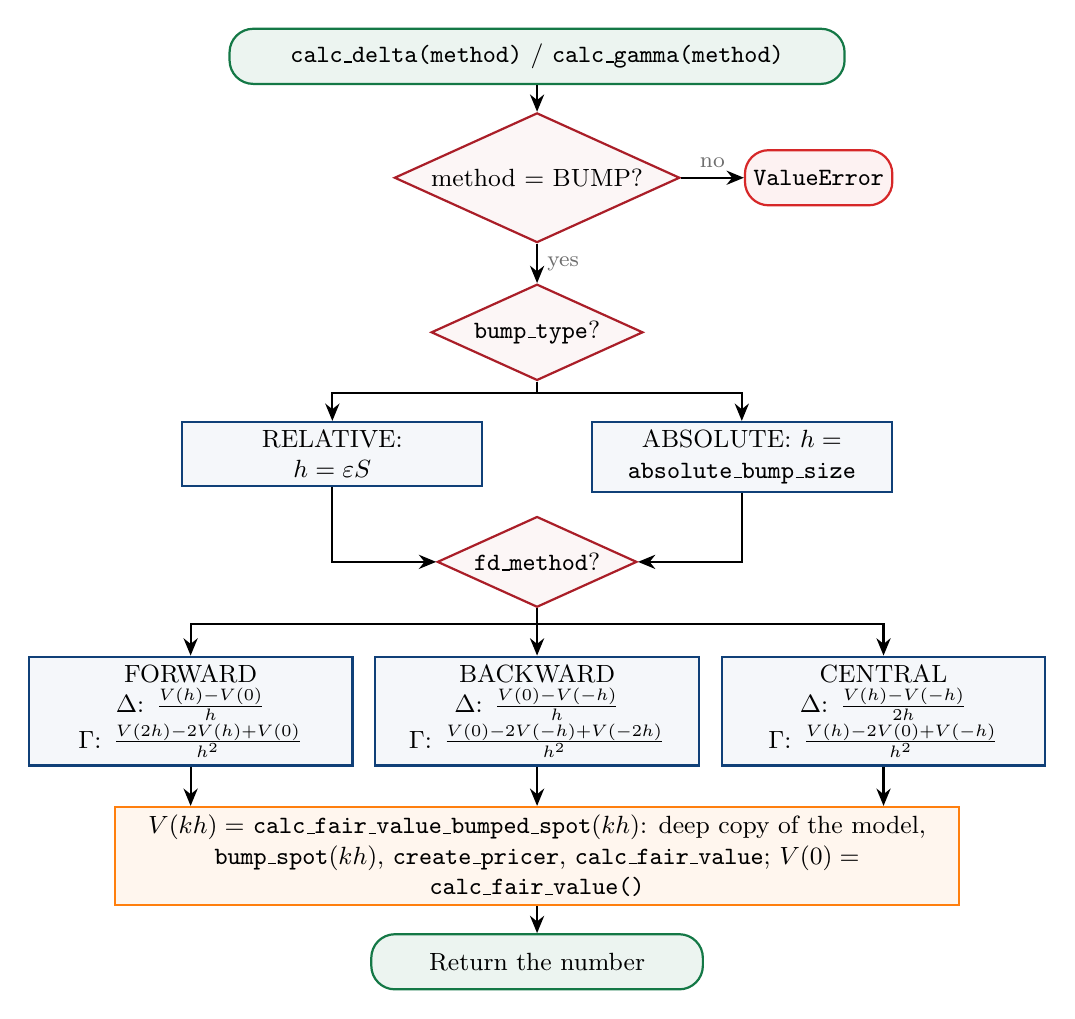
\begin{tikzpicture}[node distance=3.4mm]
\node[fcterm, text width=7.6cm] (in) {\texttt{calc\_delta(method)} / \texttt{calc\_gamma(method)}};
\node[fcdec, below=of in] (q) {method $=$ BUMP?};
\node[fcerr, right=8mm of q] (e) {\texttt{ValueError}};
\node[fcdec, below=5mm of q] (b) {\texttt{bump\_type}?};
\node[fcbox, text width=3.6cm, below=5mm of b, xshift=-2.6cm] (hr) {RELATIVE:\\ $h=\varepsilon S$};
\node[fcbox, text width=3.6cm, below=5mm of b, xshift=2.6cm] (ha) {ABSOLUTE: $h=$\\ \texttt{absolute\_bump\_size}};
\node[fcdec, below=17mm of b] (m) {\texttt{fd\_method}?};
\node[fcbox, text width=3.9cm, below=6mm of m, xshift=-4.4cm] (f) {FORWARD\\ $\Delta$: $\frac{V(h)-V(0)}{h}$\\ $\Gamma$: $\frac{V(2h)-2V(h)+V(0)}{h^2}$};
\node[fcbox, text width=3.9cm, below=6mm of m] (bk) {BACKWARD\\ $\Delta$: $\frac{V(0)-V(-h)}{h}$\\ $\Gamma$: $\frac{V(0)-2V(-h)+V(-2h)}{h^2}$};
\node[fcbox, text width=3.9cm, below=6mm of m, xshift=4.4cm] (c) {CENTRAL\\ $\Delta$: $\frac{V(h)-V(-h)}{2h}$\\ $\Gamma$: $\frac{V(h)-2V(0)+V(-h)}{h^2}$};
\node[fccall, text width=10.5cm, below=5mm of bk] (v) {$V(kh)=$ \texttt{calc\_fair\_value\_bumped\_spot}$(kh)$: deep copy of the model, \texttt{bump\_spot}$(kh)$, \texttt{create\_pricer}, \texttt{calc\_fair\_value}; $V(0)=$ \texttt{calc\_fair\_value()}};
\node[fcterm, text width=4cm, below=of v] (out) {Return the number};
\draw[fcarr] (in) -- (q); \draw[fcarr] (q) -- node[fclab, above] {no} (e); \draw[fcarr] (q) -- node[fclab, right] {yes} (b);
\draw[fcarr] (b.south) -- ++(0,-1.5mm) -| (hr.north); \draw[fcarr] (b.south) -- ++(0,-1.5mm) -| (ha.north);
\draw[fcarr] (hr.south) |- (m.west); \draw[fcarr] (ha.south) |- (m.east);
\draw[fcarr] (m.south) -- ++(0,-2mm) -| (f.north); \draw[fcarr] (m) -- (bk); \draw[fcarr] (m.south) -- ++(0,-2mm) -| (c.north);
\draw[fcarr] (f.south) -- (f.south |- v.north); \draw[fcarr] (bk) -- (v); \draw[fcarr] (c.south) -- (c.south |- v.north);
\draw[fcarr] (v) -- (out);
\end{tikzpicture}
\captionof{figure}{Flowchart of the NEW \texttt{calc\_delta} and \texttt{calc\_gamma} (another label raises \texttt{ValueError}).}
\label{fig:flowpricer}
\end{minipage}\end{center}
\hwBlocks{2}{(b), the NEW VERSION of \texttt{Pricer}}

\step{(c) Test of the new code.} Before we study the errors we test the new code. In the file \texttt{q1\_fd\_greeks\_demo.py} we first check that the defaults give the lecture's numbers; then we run the six combinations on the running example, we check two consequences of Lemma~2, we compare a class variable with an instance attribute, and we try a wrong label.
\begin{lstlisting}[style=pysmall]
# Homework 4: numerical delta and gamma with every finite difference method and bump type (running example).
# Run from this folder with the course venv:  python q1_fd_greeks_demo.py   (printed output: q1_fd_greeks_demo.out)
import sys
from pathlib import Path

here = Path(__file__).resolve().parent
sys.path.insert(0, str(here))                                   # the library of this folder
repo_root = next(p for p in [here, *here.parents] if (p / 'mkt' / 'spot.csv').exists())

from market_data import MarketData
MarketData.market_folder = repo_root / 'mkt'                    # csv files of the repository (Lecture 6)
MarketData.initialize()
from pricer import *                                            # library of Lecture 6 + NEW VERSION of Pricer

# running example: ATM 1Y call on BLUECHIP_BANK, FlatVol model (Lecture 6, cell 22)
und = Stock.BLUECHIP_BANK
spot = MarketData.get_spot()[und]
call = EuropeanContract(und, PutCallFwd.CALL, LongShort.LONG, spot, 1.0)
pricer = EuropeanAnalyticPricer(call, FlatVolModel(und), Params())
delta, gamma = pricer.calc_delta(GreekMethod.ANALYTIC), pricer.calc_gamma(GreekMethod.ANALYTIC)
print(f'ATM call: S = K = {spot}, T = 1, vol = {pricer.model.get_vol(spot, 1.0):.6f}, '
      f'value = {pricer.calc_fair_value():.6f}')
print(f'analytic: delta = {delta:.6f}, gamma = {gamma:.6f}')

# 1. default class variables = the lecture's choice (central, relative 1%): same numbers as the lecture
print(f'\ndefault: {Pricer.fd_method.value}, {Pricer.bump_type.value}, '
      f'relative_bump_size = {Pricer.relative_bump_size}')
d_bump, g_bump = pricer.calc_delta(GreekMethod.BUMP), pricer.calc_gamma(GreekMethod.BUMP)
print(f'bump: delta = {d_bump:.6f}, gamma = {g_bump:.6f}   (lecture: 0.626132, 0.007642)')
assert round(d_bump, 6) == 0.626132 and round(g_bump, 6) == 0.007642

# 2. the six combinations: relative 1% (h = 1.3017) and absolute h = 1
print(f"\n{'method':9s}{'bump':9s}{'h':>8s}{'delta':>11s}{'error':>11s}{'gamma':>11s}{'error':>11s}")
results = {}
for bump_type in BumpType:
    for fd_method in FDMethod:
        Pricer.fd_method, Pricer.bump_type = fd_method, bump_type     # class variables: used by every pricer
        h = pricer.calc_spot_bump_size()
        d, g = pricer.calc_delta(GreekMethod.BUMP), pricer.calc_gamma(GreekMethod.BUMP)
        results[fd_method, bump_type] = (d, g)
        print(f'{fd_method.value:9s}{bump_type.value:9s}{h:8.4f}{d:11.6f}{d - delta:11.2e}{g:11.6f}{g - gamma:11.2e}')
Pricer.fd_method, Pricer.bump_type = FDMethod.CENTRAL, BumpType.RELATIVE  # back to the default

# 3. checks: (forward + backward) / 2 = central for delta; forward and backward delta errors ~ +- h/2 * gamma
for bump_type in BumpType:
    fwd, bwd, cen = (results[m, bump_type][0] for m in FDMethod)
    h = Pricer.relative_bump_size * spot if bump_type == BumpType.RELATIVE else Pricer.absolute_bump_size
    print(f'{bump_type.value:9s}(fwd + bwd)/2 - central = {(fwd + bwd) / 2 - cen: .1e};  '
          f'fwd error = {fwd - delta:.6f}, h/2 * gamma = {h / 2 * gamma:.6f}')
    assert abs((fwd + bwd) / 2 - cen) < 1e-12

# 4. one pricer only: an instance attribute hides the class variable
pricer.fd_method = FDMethod.FORWARD
other = EuropeanAnalyticPricer(call, FlatVolModel(und), Params())
print(f'\ninstance: {pricer.fd_method.value}, other pricer: {other.fd_method.value}, class: {Pricer.fd_method.value}')
del pricer.fd_method

# 5. a wrong label is refused
Pricer.fd_method = 'SIDEWAYS'
try:
    pricer.calc_delta(GreekMethod.BUMP)
except ValueError as error:
    print('error:', error)
Pricer.fd_method = FDMethod.CENTRAL
\end{lstlisting}
\begin{lstlisting}[style=out]
ATM call: S = K = 130.17, T = 1, vol = 0.380830, value = 22.515663
analytic: delta = 0.626163, gamma = 0.007642

default: CENTRAL, RELATIVE, relative_bump_size = 0.01
bump: delta = 0.626132, gamma = 0.007642   (lecture: 0.626132, 0.007642)

method   bump            h      delta      error      gamma      error
FORWARD  ABSOLUTE   1.0000   0.629966   3.80e-03   0.007533  -1.09e-04
BACKWARD ABSOLUTE   1.0000   0.622324  -3.84e-03   0.007750   1.08e-04
CENTRAL  ABSOLUTE   1.0000   0.626145  -1.80e-05   0.007642  -6.19e-08
FORWARD  RELATIVE   1.3017   0.631106   4.94e-03   0.007500  -1.42e-04
BACKWARD RELATIVE   1.3017   0.621159  -5.00e-03   0.007782   1.40e-04
CENTRAL  RELATIVE   1.3017   0.626132  -3.06e-05   0.007642  -1.05e-07
ABSOLUTE (fwd + bwd)/2 - central =  0.0e+00;  fwd error = 0.003803, h/2 * gamma = 0.003821
RELATIVE (fwd + bwd)/2 - central =  0.0e+00;  fwd error = 0.004943, h/2 * gamma = 0.004974

instance: FORWARD, other pricer: CENTRAL, class: CENTRAL
error: Unsupported FDMethod SIDEWAYS
\end{lstlisting}
\noindent Reading the output: the defaults reproduce the lecture ($0.626132$, $0.007642$), so the old results are safe. With the same $h$, the central error is about $100$ times smaller than the one-sided ones, as Lemma~2 announces. Because the forward and backward delta errors are $+\frac h2\Gamma$ and $-\frac h2\Gamma$, they have opposite signs and the same size ($0.004943$ against the predicted $0.004974$ for $h=1.3017$), and their average is exactly the central difference, since the $V(0)$ terms cancel. Finally, setting \texttt{Pricer.fd\_method} changes every pricer, whereas an attribute set on one pricer changes only that one; this is how we are going to switch schemes in the study.

\begin{center}\begin{minipage}{\linewidth}\centering
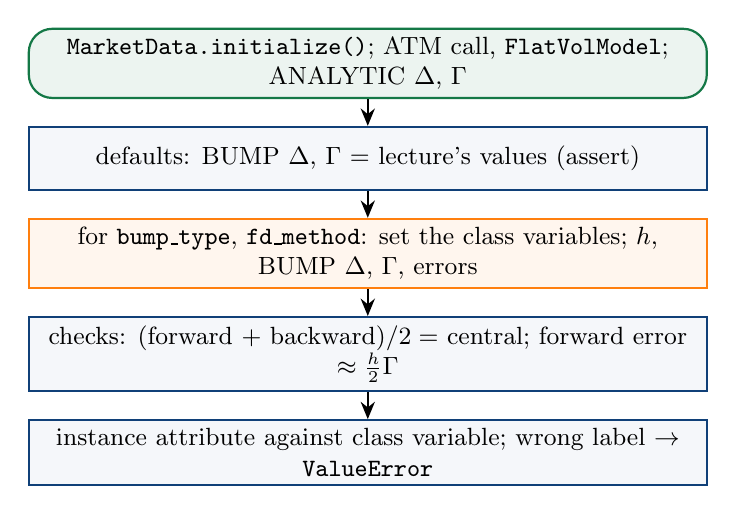
\begin{tikzpicture}[node distance=3.4mm]
\node[fcterm, text width=8.4cm] (a) {\texttt{MarketData.initialize()}; ATM call, \texttt{FlatVolModel}; ANALYTIC $\Delta$, $\Gamma$};
\node[fcbox, text width=8.4cm, below=of a] (b) {defaults: BUMP $\Delta$, $\Gamma$ $=$ lecture's values (assert)};
\node[fccall, text width=8.4cm, below=of b] (c) {for \texttt{bump\_type}, \texttt{fd\_method}: set the class variables; $h$, BUMP $\Delta$, $\Gamma$, errors};
\node[fcbox, text width=8.4cm, below=of c] (d) {checks: (forward $+$ backward)$/2=$ central; forward error $\approx\frac h2\Gamma$};
\node[fcbox, text width=8.4cm, below=of d] (e) {instance attribute against class variable; wrong label $\to$ \texttt{ValueError}};
\foreach \x/\y in {a/b,b/c,c/d,d/e} \draw[fcarr] (\x) -- (\y);
\end{tikzpicture}
\captionof{figure}{Flowchart of \texttt{q1\_fd\_greeks\_demo.py}.}
\end{minipage}\end{center}
\hwBlocks{3}{(c), \texttt{q1\_fd\_greeks\_demo.py}}

\step{(d) The comparison.} Now we can compare. In \texttt{q1\_bump\_study.py} we measure the relative error $|\text{BUMP}-\text{ANALYTIC}|/|\text{ANALYTIC}|$, so that delta and gamma, calls and puts, cheap and expensive stocks are on one scale. In Part 1 we take the running example and $17$ relative bumps $\varepsilon=10^{-1},10^{-1.5},\dots,10^{-9}$, for the three methods. In Part 2 we build a set of $72$ European options: all four stocks of \texttt{mkt/} $\times$ CALL, PUT $\times$ $K/S=0.9,1,1.1$ $\times$ $T=0.5,1,2$ (\texttt{FlatVolModel}); for every method, bump type and bump size we record the worst error over the options of each stock (absolute bumps $h=10^{1},\dots,10^{-7}$, the same range as $\varepsilon S$). In Part 3 we pick the bump with the smallest worst error.
\begin{lstlisting}[style=pysmall]
# Homework 4: error of the numerical delta and gamma against the bump size, for every finite difference method;
# absolute against relative bumping on a set of European options; suggested (optimal) bump sizes.
# Run from this folder with the course venv:  python q1_bump_study.py   (output: q1_bump_study.out, figures/)
import sys
from pathlib import Path

here = Path(__file__).resolve().parent
sys.path.insert(0, str(here))                                   # the library of this folder
repo_root = next(p for p in [here, *here.parents] if (p / 'mkt' / 'spot.csv').exists())

import matplotlib
matplotlib.use('Agg')                                           # files only (no window)
import matplotlib.pyplot as plt
import numpy as np
from market_data import MarketData
MarketData.market_folder = repo_root / 'mkt'
MarketData.initialize()
from pricer import *                                            # library of Lecture 6 + NEW VERSION of Pricer

(here / 'figures').mkdir(exist_ok=True)
sizes = 10.0 ** -np.arange(1.0, 9.01, 0.5)                      # relative bumps eps = 1e-1, ..., 1e-9 (17 values)
abs_sizes = 10.0 ** -np.arange(-1.0, 7.01, 0.5)                 # absolute bumps h = 1e1, ..., 1e-7 (17 values)
greeks = ('delta', 'gamma')


def set_bump(fd_method: FDMethod, bump_type: BumpType, size: float) -> None:
    Pricer.fd_method, Pricer.bump_type = fd_method, bump_type   # class variables: used by every pricer
    if bump_type == BumpType.RELATIVE:
        Pricer.relative_bump_size = size
    else:
        Pricer.absolute_bump_size = size


def rel_error(pricer: Pricer, greek: str) -> float:
    exact = getattr(pricer, f'calc_{greek}')(GreekMethod.ANALYTIC)
    return abs(getattr(pricer, f'calc_{greek}')(GreekMethod.BUMP) - exact) / abs(exact)


# 1. ATM 1Y call on BLUECHIP_BANK (running example): relative error against eps, 3 methods
und = Stock.BLUECHIP_BANK
spot = MarketData.get_spot()[und]
atm = EuropeanAnalyticPricer(EuropeanContract(und, PutCallFwd.CALL, LongShort.LONG, spot, 1.0),
                             FlatVolModel(und), Params())
atm_err = {}
for fd_method in FDMethod:
    for greek in greeks:
        errs = []
        for eps in sizes:
            set_bump(fd_method, BumpType.RELATIVE, eps)
            errs.append(rel_error(atm, greek))
        atm_err[fd_method, greek] = np.array(errs)
print('1. ATM call, relative bump: relative error of delta | gamma')
print('eps     ' + ''.join(f'{m.value:>10s}' for m in FDMethod) + ' |' + ''.join(f'{m.value:>10s}' for m in FDMethod))
for i, eps in enumerate(sizes):
    print(f'{eps:7.0e} ' + ''.join(f'{atm_err[m, "delta"][i]:10.1e}' for m in FDMethod) + ' |'
          + ''.join(f'{atm_err[m, "gamma"][i]:10.1e}' for m in FDMethod))
for greek in greeks:                                            # slope of log(error) on eps in [1e-3, 1e-1]
    slopes = [np.polyfit(np.log10(sizes[:5]), np.log10(atm_err[m, greek][:5]), 1)[0] for m in FDMethod]
    print(f'slopes {greek}: ' + ', '.join(f'{m.value} {s:.2f}' for m, s in zip(FDMethod, slopes)))

# 2. the set of European options: 4 stocks x CALL, PUT x K/S = 0.9, 1, 1.1 x T = 0.5, 1, 2 (72 options)
book = [EuropeanAnalyticPricer(EuropeanContract(s, cp, LongShort.LONG, k * MarketData.get_spot()[s], t),
                               FlatVolModel(s), Params())
        for s in Stock for cp in (PutCallFwd.CALL, PutCallFwd.PUT) for k in (0.9, 1.0, 1.1) for t in (0.5, 1.0, 2.0)]
worst = {}                                                      # worst relative error over the options of a stock
for bump_type, grid in ((BumpType.RELATIVE, sizes), (BumpType.ABSOLUTE, abs_sizes)):
    for fd_method in FDMethod:
        for greek in greeks:
            table = np.zeros((len(Stock), len(grid)))
            for j, size in enumerate(grid):
                set_bump(fd_method, bump_type, size)
                for i, stock in enumerate(Stock):
                    table[i, j] = max(rel_error(p, greek) for p in book if p.contract.underlying == stock)
            worst[bump_type, fd_method, greek] = table
set_bump(FDMethod.CENTRAL, BumpType.RELATIVE, 0.01)             # back to the lecture's default
Pricer.absolute_bump_size = 1.0

# 3. suggested bump sizes: the grid value with the smallest worst error over all 72 options
print(f'\n2. {len(book)} options; suggested bumps (worst relative error over the set at that bump)')
print(f"{'greek':6s}{'method':9s}{'relative eps*':>14s}{'error':>9s}{'absolute h*':>13s}{'error':>9s}"
      + ''.join(f'{"h* " + s.value[:8]:>13s}' for s in Stock))
for greek in greeks:
    for fd_method in FDMethod:
        rel = worst[BumpType.RELATIVE, fd_method, greek].max(axis=0)
        ab = worst[BumpType.ABSOLUTE, fd_method, greek]
        per_stock = [abs_sizes[int(np.argmin(row))] for row in ab]
        print(f'{greek:6s}{fd_method.value:9s}{sizes[int(np.argmin(rel))]:14.0e}{rel.min():9.1e}'
              f'{abs_sizes[int(np.argmin(ab.max(axis=0)))]:13.0e}{ab.max(axis=0).min():9.1e}'
              + ''.join(f'{h:13.0e}' for h in per_stock))
print('spots: ' + ', '.join(f'{s.value} {MarketData.get_spot()[s]}' for s in Stock))
for greek in greeks:                                            # the relative eps* does not depend on the stock
    rows = worst[BumpType.RELATIVE, FDMethod.CENTRAL, greek]
    print(f'central {greek}, relative eps* per stock: ' + ', '.join(f'{sizes[int(np.argmin(r))]:.0e}' for r in rows))

# one relative bump for both greeks (the library has one relative_bump_size): central differences
both = np.maximum(worst[BumpType.RELATIVE, FDMethod.CENTRAL, 'delta'].max(axis=0),
                  worst[BumpType.RELATIVE, FDMethod.CENTRAL, 'gamma'].max(axis=0))
best = int(np.argmin(both))
lecture = int(np.argmin(abs(sizes - 0.01)))
print(f'central, one eps for delta and gamma: eps* = {sizes[best]:.0e}, worst error {both[best]:.1e}  '
      f'(lecture eps = 1e-02: {both[lecture]:.1e})')

# 4. data for the figures of the report (csv) and the figures (png)
np.savetxt(here / 'figures' / 'atm_errors.csv',
           np.column_stack([sizes] + [atm_err[m, g] for g in greeks for m in FDMethod]), delimiter=',',
           header='eps,' + ','.join(f'{g}_{m.value}' for g in greeks for m in FDMethod), comments='')
for bump_type, grid in ((BumpType.RELATIVE, sizes), (BumpType.ABSOLUTE, abs_sizes)):
    for greek in greeks:
        np.savetxt(here / 'figures' / f'worst_{greek}_{bump_type.value.lower()}_central.csv',
                   np.column_stack([grid, worst[bump_type, FDMethod.CENTRAL, greek].T]), delimiter=',',
                   header='size,' + ','.join(s.value for s in Stock), comments='')

fig, axes = plt.subplots(1, 2, figsize=(11, 4))
for ax, greek in zip(axes, greeks):
    for m, mark in zip(FDMethod, 'o^s'):
        ax.loglog(sizes, atm_err[m, greek], marker=mark, label=m.value.lower())
    ax.set_title(f'{greek}: ATM 1Y call, BLUECHIP_BANK, relative bump')
    ax.set_xlabel('relative bump eps (h = eps * S)')
    ax.set_ylabel('relative error')
    ax.grid(True, which='major', ls=':')
    ax.legend()
fig.tight_layout()
fig.savefig(here / 'figures' / 'q1_error_vs_bump.png', dpi=150)
fig, axes = plt.subplots(2, 2, figsize=(11, 7.5))
for row, greek in enumerate(greeks):
    for col, (bump_type, grid) in enumerate(((BumpType.ABSOLUTE, abs_sizes), (BumpType.RELATIVE, sizes))):
        ax = axes[row, col]
        for i, s in enumerate(Stock):
            ax.loglog(grid, worst[bump_type, FDMethod.CENTRAL, greek][i], marker='o', ms=3,
                      label=f'{s.value} (S = {MarketData.get_spot()[s]})')
        ax.set_title(f'central {greek}, {bump_type.value.lower()} bump: worst error per stock')
        ax.set_xlabel('h' if bump_type == BumpType.ABSOLUTE else 'eps (h = eps * S)')
        ax.set_ylabel('worst relative error')
        ax.grid(True, which='major', ls=':')
        ax.legend(fontsize=7)
fig.tight_layout()
fig.savefig(here / 'figures' / 'q1_absolute_vs_relative.png', dpi=150)
print('figures saved in figures/')
\end{lstlisting}
\begin{lstlisting}[style=outsmall]
1. ATM call, relative bump: relative error of delta | gamma
eps        FORWARD  BACKWARD   CENTRAL |   FORWARD  BACKWARD   CENTRAL
  1e-01    7.4e-02   8.4e-02   4.8e-03 |   1.9e-01   1.6e-01   1.4e-03
  3e-02    2.5e-02   2.6e-02   4.9e-04 |   5.9e-02   5.7e-02   1.4e-04
  1e-02    7.9e-03   8.0e-03   4.9e-05 |   1.9e-02   1.8e-02   1.4e-05
  3e-03    2.5e-03   2.5e-03   4.9e-06 |   5.8e-03   5.8e-03   1.4e-06
  1e-03    7.9e-04   7.9e-04   4.9e-07 |   1.8e-03   1.8e-03   1.4e-07
  3e-04    2.5e-04   2.5e-04   4.9e-08 |   5.8e-04   5.8e-04   1.3e-08
  1e-04    7.9e-05   7.9e-05   4.9e-09 |   1.8e-04   1.8e-04   5.0e-09
  3e-05    2.5e-05   2.5e-05   4.9e-10 |   5.8e-05   5.8e-05   1.3e-07
  1e-05    7.9e-06   7.9e-06   5.6e-11 |   1.9e-05   1.7e-05   1.1e-06
  3e-06    2.5e-06   2.5e-06   2.7e-11 |   1.4e-05   1.9e-05   8.2e-06
  1e-06    7.9e-07   7.9e-07   8.8e-13 |   4.1e-05   6.9e-05   4.1e-05
  3e-07    2.5e-07   2.5e-07   1.7e-10 |   1.8e-04   1.8e-04   3.7e-04
  1e-07    7.9e-08   8.2e-08   1.7e-09 |   2.1e-02   2.3e-02   9.7e-03
  3e-08    2.8e-08   2.5e-08   1.7e-09 |   1.2e-01   9.7e-02   4.3e-02
  1e-08    2.0e-08   6.0e-09   7.1e-09 |   1.5e+00   6.5e-01   6.5e-01
  3e-09    4.7e-08   8.0e-09   2.0e-08 |   1.7e+01   4.5e+00   1.0e+01
  1e-09    2.4e-07   6.4e-08   1.5e-07 |   3.9e+02   2.2e+02   1.1e+02
slopes delta: FORWARD 0.99, BACKWARD 1.01, CENTRAL 2.00
slopes gamma: FORWARD 1.00, BACKWARD 0.98, CENTRAL 2.01

2. 72 options; suggested bumps (worst relative error over the set at that bump)
greek method    relative eps*    error  absolute h*    error  h* TEST_COM  h* BLUECHIP  h* TIPTOP_S  h* MONEY_MA
delta FORWARD           1e-08  6.7e-08        3e-06  7.9e-08        1e-06        1e-06        1e-06        3e-06
delta BACKWARD          1e-08  5.3e-08        3e-06  8.2e-08        1e-06        1e-06        1e-06        3e-06
delta CENTRAL           3e-06  8.0e-11        3e-04  1.3e-10        3e-04        3e-04        1e-03        1e-03
gamma FORWARD           1e-05  3.8e-05        1e-03  3.8e-05        3e-04        1e-03        1e-03        3e-03
gamma BACKWARD          1e-05  4.1e-05        1e-03  4.1e-05        3e-04        1e-03        1e-03        1e-03
gamma CENTRAL           1e-04  4.1e-08        3e-02  1.4e-07        1e-02        1e-02        1e-02        3e-02
spots: TEST_COMPANY 100.0, BLUECHIP_BANK 130.17, TIPTOP_SOLUTIONS 177.32, MONEY_MALL 250.86
central delta, relative eps* per stock: 3e-06, 3e-06, 3e-06, 3e-06
central gamma, relative eps* per stock: 1e-04, 1e-04, 1e-04, 1e-04
central, one eps for delta and gamma: eps* = 1e-04, worst error 4.1e-08  (lecture eps = 1e-02: 3.2e-04)
figures saved in figures/
\end{lstlisting}

\begin{center}\begin{minipage}{\linewidth}\centering
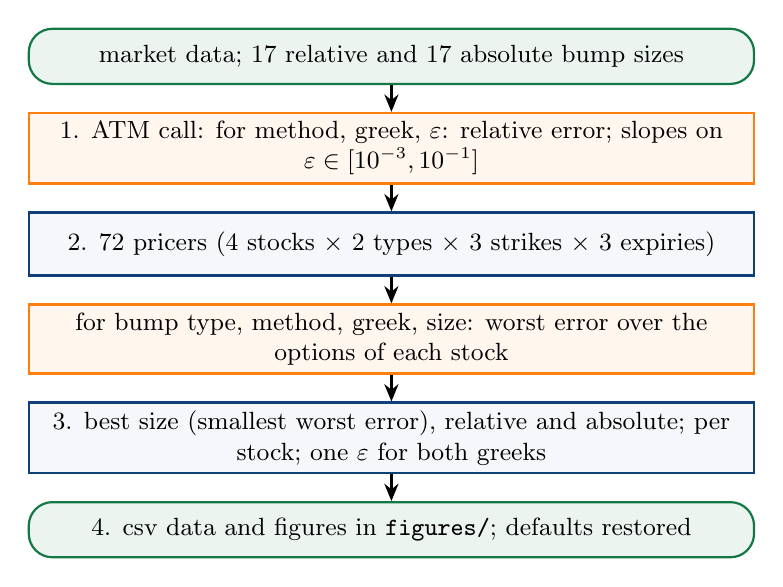
\begin{tikzpicture}[node distance=3.4mm]
\node[fcterm, text width=9cm] (a) {market data; 17 relative and 17 absolute bump sizes};
\node[fccall, text width=9cm, below=of a] (b) {1. ATM call: for method, greek, $\varepsilon$: relative error; slopes on $\varepsilon\in[10^{-3},10^{-1}]$};
\node[fcbox, text width=9cm, below=of b] (c) {2. 72 pricers (4 stocks $\times$ 2 types $\times$ 3 strikes $\times$ 3 expiries)};
\node[fccall, text width=9cm, below=of c] (d) {for bump type, method, greek, size: worst error over the options of each stock};
\node[fcbox, text width=9cm, below=of d] (e) {3. best size (smallest worst error), relative and absolute; per stock; one $\varepsilon$ for both greeks};
\node[fcterm, text width=9cm, below=of e] (f) {4. csv data and figures in \texttt{figures/}; defaults restored};
\foreach \x/\y in {a/b,b/c,c/d,d/e,e/f} \draw[fcarr] (\x) -- (\y);
\end{tikzpicture}
\captionof{figure}{Flowchart of \texttt{q1\_bump\_study.py}.}
\end{minipage}\end{center}
\hwBlocks{4}{(d), \texttt{q1\_bump\_study.py}: all blocks of the homework}

% =====================================================================
\subhead{5. Results.}
\step{The numerical error.} We look first at the running example (Figure~\ref{fig:atm}).
\begin{center}\begin{minipage}{\linewidth}\centering
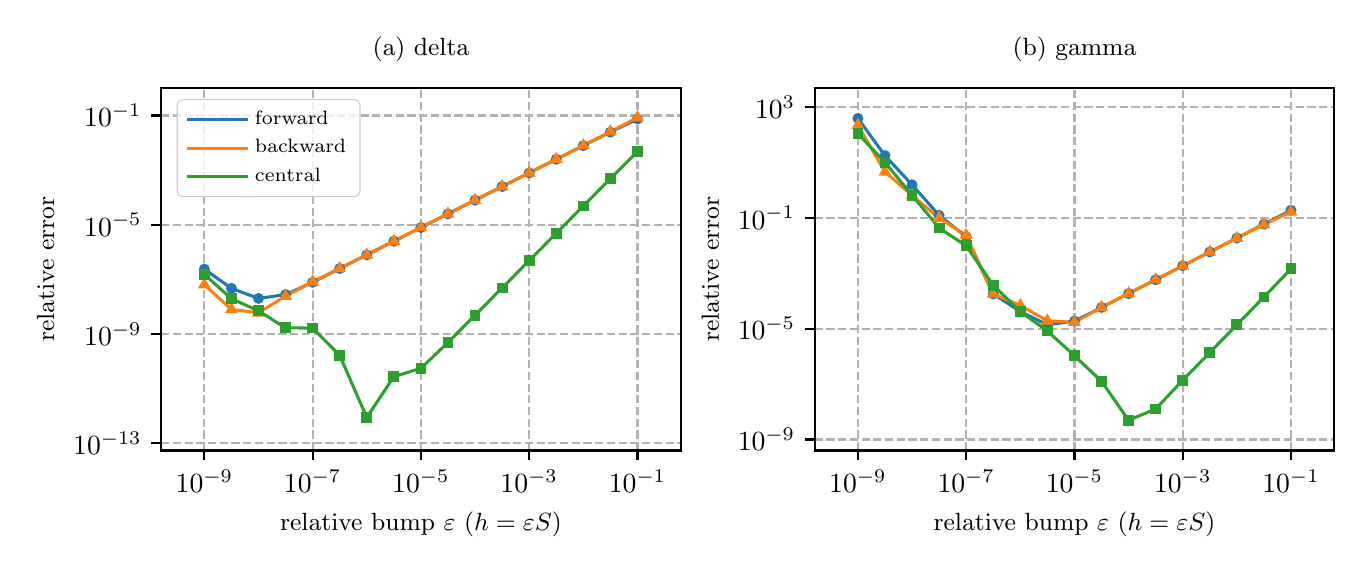
\begin{tikzpicture}
\begin{axis}[mpl, mplgrid, xmode=log, ymode=log, width=6.6cm, height=4.6cm, title={(a) delta}, xlabel={relative bump $\varepsilon$ ($h=\varepsilon S$)}, xtick={1e-9,1e-7,1e-5,1e-3,1e-1},
  ylabel={relative error}, legend pos=north west, legend style={font=\scriptsize}, title style={font=\small}, label style={font=\small}, ymax=1]
\addplot[tabblue, line width=1.1pt, mark=*, mark size=1.4pt] coordinates {(0.1,0.074484) (0.0316228,0.0246268) (0.01,0.00789411) (0.00316228,0.00250693) (0.001,0.000793818) (0.000316228,0.000251133) (0.0001,7.94257e-05) (3.16228e-05,2.51177e-05) (1e-05,7.94301e-06) (3.16228e-06,2.51186e-06) (1e-06,7.9434e-07) (3.16228e-07,2.5144e-07) (1e-07,7.85456e-08) (3.16228e-08,2.78703e-08) (1e-08,2.01383e-08) (3.16228e-09,4.71673e-08) (1e-09,2.38076e-07)}; \addlegendentry{forward}
\addplot[taborange, line width=1.1pt, mark=triangle*, mark size=1.6pt] coordinates {(0.1,0.0841502) (0.0316228,0.0256026) (0.01,0.00799179) (0.00316228,0.0025167) (0.001,0.000794794) (0.000316228,0.000251231) (0.0001,7.94355e-05) (3.16228e-05,2.51187e-05) (1e-05,7.94313e-06) (3.16228e-06,2.51181e-06) (1e-06,7.94338e-07) (3.16228e-07,2.51109e-07) (1e-07,8.18565e-08) (3.16228e-08,2.45073e-08) (1e-08,6.01419e-09) (3.16228e-09,7.96698e-09) (1e-09,6.37258e-08)}; \addlegendentry{backward}
\addplot[tabgreen, line width=1.1pt, mark=square*, mark size=1.4pt] coordinates {(0.1,0.00483308) (0.0316228,0.000487921) (0.01,4.88382e-05) (0.00316228,4.88428e-06) (0.001,4.88432e-07) (0.000316228,4.8843e-08) (0.0001,4.88528e-09) (3.16228e-05,4.92147e-10) (1e-05,5.57797e-11) (3.16228e-06,2.74946e-11) (1e-06,8.84047e-13) (3.16228e-07,1.65331e-10) (1e-07,1.65544e-09) (3.16228e-08,1.68152e-09) (1e-08,7.06206e-09) (3.16228e-09,1.96002e-08) (1e-09,1.50901e-07)}; \addlegendentry{central}
\end{axis}
\begin{axis}[mpl, mplgrid, xmode=log, ymode=log, at={(8.3cm,0)}, width=6.6cm, height=4.6cm, title={(b) gamma}, xlabel={relative bump $\varepsilon$ ($h=\varepsilon S$)}, xtick={1e-9,1e-7,1e-5,1e-3,1e-1},
  ylabel={relative error}, title style={font=\small}, label style={font=\small}]
\addplot[tabblue, line width=1.1pt, mark=*, mark size=1.4pt] coordinates {(0.1,0.186094) (0.0316228,0.0590088) (0.01,0.0185341) (0.00316228,0.00584292) (0.001,0.0018457) (0.000316228,0.00058346) (0.0001,0.000184468) (3.16228e-05,5.8371e-05) (1e-05,1.86964e-05) (3.16228e-06,1.37577e-05) (1e-06,4.11173e-05) (3.16228e-07,0.000178383) (1e-07,0.0206741) (3.16228e-08,0.122001) (1e-08,1.54875) (3.16228e-09,17.4625) (1e-09,385.125)};
\addplot[taborange, line width=1.1pt, mark=triangle*, mark size=1.6pt] coordinates {(0.1,0.163447) (0.0316228,0.0570519) (0.01,0.0183416) (0.00316228,0.0058237) (0.001,0.00184378) (0.000316228,0.000583266) (0.0001,0.000184445) (3.16228e-05,5.81834e-05) (1e-05,1.69723e-05) (3.16228e-06,1.91673e-05) (1e-06,6.86326e-05) (3.16228e-07,0.000178383) (1e-07,0.0232259) (3.16228e-08,0.097499) (1e-08,0.646249) (3.16228e-09,4.4875) (1e-09,218.5)};
\addplot[tabgreen, line width=1.1pt, mark=square*, mark size=1.4pt] coordinates {(0.1,0.00142926) (0.0316228,0.000137835) (0.01,1.37323e-05) (0.00316228,1.37272e-06) (0.001,1.37107e-07) (0.000316228,1.25959e-08) (0.0001,4.9641e-09) (3.16228e-05,1.25689e-07) (1e-05,1.05856e-06) (3.16228e-06,8.19231e-06) (1e-06,4.11173e-05) (3.16228e-07,0.000370367) (1e-07,0.00969911) (3.16228e-08,0.0426241) (1e-08,0.646249) (3.16228e-09,9.97499) (1e-09,108.75)};
\end{axis}
\end{tikzpicture}
\captionof{figure}{Relative error of the numerical delta and gamma of the running example (ATM 1Y call, \texttt{BLUECHIP\_BANK}, relative bump). Right part: truncation, slope $1$ (forward, backward) and $2$ (central); left part: rounding. Same numbers as \texttt{figures/q1\_error\_vs\_bump.png}.}
\label{fig:atm}
\end{minipage}\end{center}
\noindent On the right of the figure the slopes are $0.99$, $1.01$, $2.00$ (delta) and $1.00$, $0.98$, $2.01$ (gamma), exactly as Lemma~2 predicts. Moving to the left, the error falls until the rounding takes over (Section~3) and then rises; for gamma, which divides by $h^2$, the rise is much steeper. At every reasonable $\varepsilon$ the central scheme is the most accurate, by orders of magnitude. The lecture's $\varepsilon=1\%$ gives $4.9\cdot10^{-5}$ (delta) and $1.4\cdot10^{-5}$ (gamma), whereas the best central bumps give about $10^{-12}$ and $5\cdot10^{-9}$.

\step{Absolute against relative bumping.} Next we compare the two bump types on the set of $72$ options, with the central scheme (Figure~\ref{fig:absrel}).
\begin{center}\begin{minipage}{\linewidth}\centering
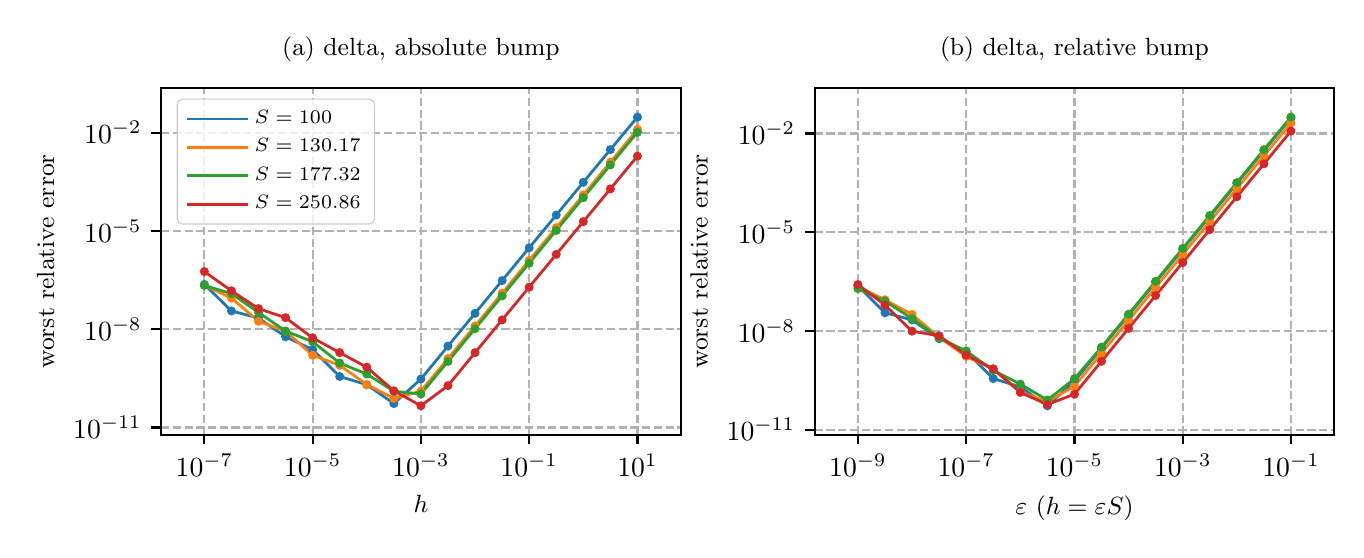
\begin{tikzpicture}
\begin{axis}[mpl, mplgrid, xmode=log, ymode=log, width=6.6cm, height=4.4cm, title={(a) delta, absolute bump}, xlabel={$h$}, xtick={1e-7,1e-5,1e-3,1e-1,1e1},
  ylabel={worst relative error}, legend pos=north west, legend style={font=\scriptsize}, title style={font=\small}, label style={font=\small}]
\addplot[tabblue, line width=1pt, mark=*, mark size=1.1pt] coordinates {(10,0.0298536) (3.16228,0.00303497) (1,0.000303993) (0.316228,3.04042e-05) (0.1,3.04047e-06) (0.0316228,3.04048e-07) (0.01,3.04052e-08) (0.00316228,3.03662e-09) (0.001,2.99665e-10) (0.000316228,5.34911e-11) (0.0001,2.00805e-10) (3.16228e-05,3.59232e-10) (1e-05,2.36409e-09) (3.16228e-06,5.85698e-09) (1e-06,2.18339e-08) (3.16228e-07,3.58893e-08) (1e-07,2.33299e-07)}; \addlegendentry{$S=100$}
\addplot[taborange, line width=1pt, mark=*, mark size=1.1pt] coordinates {(10,0.0124575) (3.16228,0.00125476) (1,0.000125566) (0.316228,1.25575e-05) (0.1,1.25576e-06) (0.0316228,1.25576e-07) (0.01,1.25571e-08) (0.00316228,1.26309e-09) (0.001,1.27746e-10) (0.000316228,7.68575e-11) (0.0001,2.03568e-10) (3.16228e-05,7.8942e-10) (1e-05,1.59475e-09) (3.16228e-06,8.66003e-09) (1e-06,1.7412e-08) (3.16228e-07,8.85959e-08) (1e-07,2.19973e-07)}; \addlegendentry{$S=130.17$}
\addplot[tabgreen, line width=1pt, mark=*, mark size=1.1pt] coordinates {(10,0.0102574) (3.16228,0.00103135) (1,0.000103191) (0.316228,1.03197e-05) (0.1,1.03198e-06) (0.0316228,1.03197e-07) (0.01,1.03191e-08) (0.00316228,1.03322e-09) (0.001,1.04703e-10) (0.000316228,1.27636e-10) (0.0001,4.25736e-10) (3.16228e-05,9.20478e-10) (1e-05,4.13342e-09) (3.16228e-06,8.74652e-09) (1e-06,3.23754e-08) (3.16228e-07,1.21377e-07) (1e-07,2.1557e-07)}; \addlegendentry{$S=177.32$}
\addplot[tabred, line width=1pt, mark=*, mark size=1.1pt] coordinates {(10,0.00191201) (3.16228,0.000191394) (1,1.91413e-05) (0.316228,1.91415e-06) (0.1,1.91415e-07) (0.0316228,1.91419e-08) (0.01,1.91454e-09) (0.00316228,1.88162e-10) (0.001,4.57256e-11) (0.000316228,1.30983e-10) (0.0001,6.89297e-10) (3.16228e-05,1.91932e-09) (1e-05,5.39891e-09) (3.16228e-06,2.23757e-08) (1e-06,4.23159e-08) (3.16228e-07,1.47823e-07) (1e-07,5.72551e-07)}; \addlegendentry{$S=250.86$}
\end{axis}
\begin{axis}[mpl, mplgrid, xmode=log, ymode=log, at={(8.3cm,0)}, width=6.6cm, height=4.4cm, title={(b) delta, relative bump}, xlabel={$\varepsilon$ ($h=\varepsilon S$)}, xtick={1e-9,1e-7,1e-5,1e-3,1e-1},
  ylabel={worst relative error}, title style={font=\small}, label style={font=\small}]
\addplot[tabblue, line width=1pt, mark=*, mark size=1.1pt] coordinates {(0.1,0.0298536) (0.0316228,0.00303497) (0.01,0.000303993) (0.00316228,3.04042e-05) (0.001,3.04047e-06) (0.000316228,3.04048e-07) (0.0001,3.04052e-08) (3.16228e-05,3.03662e-09) (1e-05,2.99665e-10) (3.16228e-06,5.34911e-11) (1e-06,2.00805e-10) (3.16228e-07,3.59232e-10) (1e-07,2.36409e-09) (3.16228e-08,5.85698e-09) (1e-08,2.18339e-08) (3.16228e-09,3.58893e-08) (1e-09,2.33299e-07)};
\addplot[taborange, line width=1pt, mark=*, mark size=1.1pt] coordinates {(0.1,0.0209901) (0.0316228,0.00212492) (0.01,0.000212751) (0.00316228,2.12776e-05) (0.001,2.12779e-06) (0.000316228,2.1278e-07) (0.0001,2.12779e-08) (3.16228e-05,2.13341e-09) (1e-05,2.11732e-10) (3.16228e-06,7.14399e-11) (1e-06,1.40718e-10) (3.16228e-07,6.91506e-10) (1e-07,1.69115e-09) (3.16228e-08,6.43258e-09) (1e-08,3.18079e-08) (3.16228e-09,8.90766e-08) (1e-09,2.23228e-07)};
\addplot[tabgreen, line width=1pt, mark=*, mark size=1.1pt] coordinates {(0.1,0.031831) (0.0316228,0.00323862) (0.01,0.000324417) (0.00316228,3.24472e-05) (0.001,3.24478e-06) (0.000316228,3.24478e-07) (0.0001,3.24473e-08) (3.16228e-05,3.24619e-09) (1e-05,3.54734e-10) (3.16228e-06,7.98953e-11) (1e-06,2.44531e-10) (3.16228e-07,6.31294e-10) (1e-07,2.4762e-09) (3.16228e-08,6.14607e-09) (1e-08,2.38945e-08) (3.16228e-09,8.10682e-08) (1e-09,1.95286e-07)};
\addplot[tabred, line width=1pt, mark=*, mark size=1.1pt] coordinates {(0.1,0.0119607) (0.0316228,0.00120374) (0.01,0.00012045) (0.00316228,1.20458e-05) (0.001,1.20459e-06) (0.000316228,1.20459e-07) (0.0001,1.20445e-08) (3.16228e-05,1.20085e-09) (1e-05,1.20574e-10) (3.16228e-06,5.84254e-11) (1e-06,1.36711e-10) (3.16228e-07,7.10347e-10) (1e-07,1.8506e-09) (3.16228e-08,7.15608e-09) (1e-08,9.8956e-09) (3.16228e-09,6.1245e-08) (1e-09,2.59822e-07)};
\end{axis}
\end{tikzpicture}

\vspace{3mm}
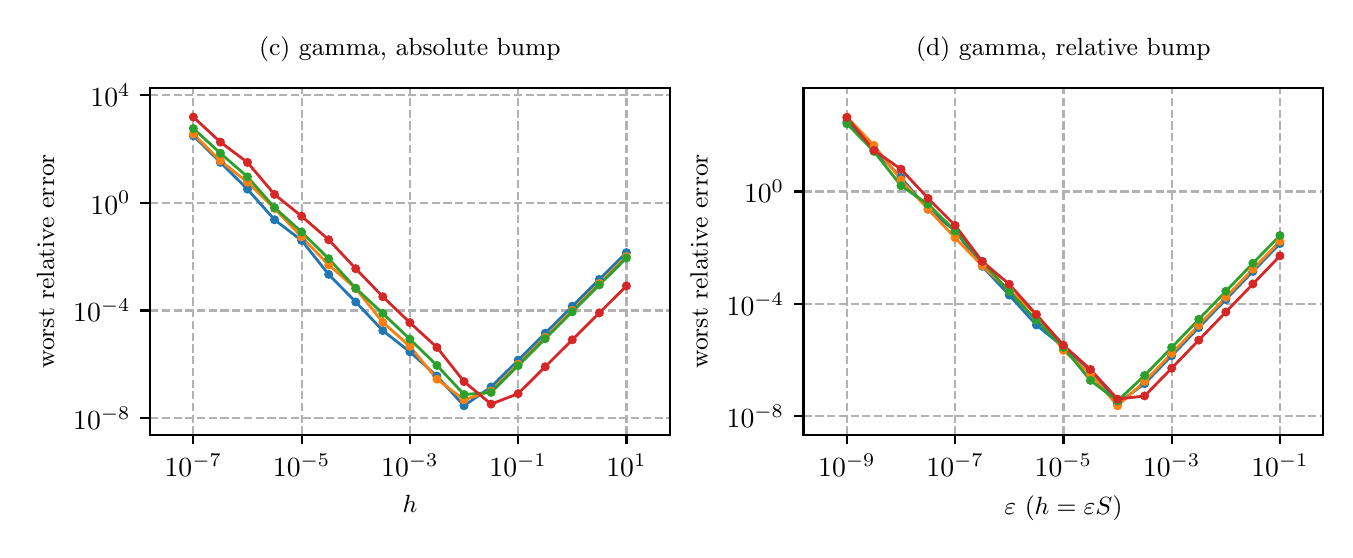
\begin{tikzpicture}
\begin{axis}[mpl, mplgrid, xmode=log, ymode=log, width=6.6cm, height=4.4cm, title={(c) gamma, absolute bump}, xlabel={$h$}, xtick={1e-7,1e-5,1e-3,1e-1,1e1},
  ylabel={worst relative error}, title style={font=\small}, label style={font=\small}]
\addplot[tabblue, line width=1pt, mark=*, mark size=1.1pt] coordinates {(10,0.0141267) (3.16228,0.00142863) (1,0.000143023) (0.316228,1.43039e-05) (0.1,1.43054e-06) (0.0316228,1.43897e-07) (0.01,2.89255e-08) (0.00316228,3.64433e-07) (0.001,2.91272e-06) (0.000316228,1.78528e-05) (0.0001,0.000206134) (3.16228e-05,0.00218118) (1e-05,0.0398302) (3.16228e-06,0.233346) (1e-06,3.18322) (3.16228e-07,31.6662) (1e-07,307.662)};
\addplot[taborange, line width=1pt, mark=*, mark size=1.1pt] coordinates {(10,0.0100435) (3.16228,0.00101336) (1,0.000101426) (0.316228,1.01435e-05) (0.1,1.01455e-06) (0.0316228,1.01872e-07) (0.01,4.81719e-08) (0.00316228,2.80326e-07) (0.001,4.66449e-06) (0.000316228,3.62362e-05) (0.0001,0.000651724) (3.16228e-05,0.00492801) (1e-05,0.0537999) (3.16228e-06,0.611813) (1e-06,5.80952) (3.16228e-07,36.1578) (1e-07,354.201)};
\addplot[tabgreen, line width=1pt, mark=*, mark size=1.1pt] coordinates {(10,0.00884679) (3.16228,0.000893185) (1,8.94043e-05) (0.316228,8.94131e-06) (0.1,8.94466e-07) (0.0316228,9.05578e-08) (0.01,7.58481e-08) (0.00316228,9.09804e-07) (0.001,8.61502e-06) (0.000316228,7.79874e-05) (0.0001,0.000665388) (3.16228e-05,0.00838516) (1e-05,0.0818381) (3.16228e-06,0.661016) (1e-06,9.16144) (3.16228e-07,68.7968) (1e-07,570.421)};
\addplot[tabred, line width=1pt, mark=*, mark size=1.1pt] coordinates {(10,0.000813982) (3.16228,8.1365e-05) (1,8.13616e-06) (0.316228,8.13689e-07) (0.1,8.18992e-08) (0.0316228,3.32877e-08) (0.01,2.29356e-07) (0.00316228,4.25562e-06) (0.001,3.54022e-05) (0.000316228,0.000324163) (0.0001,0.00356653) (3.16228e-05,0.0422901) (1e-05,0.316295) (3.16228e-06,2.03869) (1e-06,31.3869) (3.16228e-07,178.768) (1e-07,1520.35)};
\end{axis}
\begin{axis}[mpl, mplgrid, xmode=log, ymode=log, at={(8.3cm,0)}, width=6.6cm, height=4.4cm, title={(d) gamma, relative bump}, xlabel={$\varepsilon$ ($h=\varepsilon S$)}, xtick={1e-9,1e-7,1e-5,1e-3,1e-1},
  ylabel={worst relative error}, title style={font=\small}, label style={font=\small}]
\addplot[tabblue, line width=1pt, mark=*, mark size=1.1pt] coordinates {(0.1,0.0141267) (0.0316228,0.00142863) (0.01,0.000143023) (0.00316228,1.43039e-05) (0.001,1.43054e-06) (0.000316228,1.43897e-07) (0.0001,2.89255e-08) (3.16228e-05,3.64433e-07) (1e-05,2.91272e-06) (3.16228e-06,1.78528e-05) (1e-06,0.000206134) (3.16228e-07,0.00218118) (1e-07,0.0398302) (3.16228e-08,0.233346) (1e-08,3.18322) (3.16228e-09,31.6662) (1e-09,307.662)};
\addplot[taborange, line width=1pt, mark=*, mark size=1.1pt] coordinates {(0.1,0.0169007) (0.0316228,0.00171588) (0.01,0.000171847) (0.00316228,1.71873e-05) (0.001,1.71887e-06) (0.000316228,1.72419e-07) (0.0001,2.35827e-08) (3.16228e-05,3.19739e-07) (1e-05,2.21489e-06) (3.16228e-06,4.25306e-05) (1e-06,0.000303918) (3.16228e-07,0.00228686) (1e-07,0.0225203) (3.16228e-08,0.236344) (1e-08,2.60535) (3.16228e-09,44.0669) (1e-09,449.669)};
\addplot[tabgreen, line width=1pt, mark=*, mark size=1.1pt] coordinates {(0.1,0.0271941) (0.0316228,0.00280198) (0.01,0.000281044) (0.00316228,2.81129e-05) (0.001,2.81143e-06) (0.000316228,2.82835e-07) (0.0001,3.51115e-08) (3.16228e-05,1.88474e-07) (1e-05,2.82359e-06) (3.16228e-06,2.63666e-05) (1e-06,0.000273514) (3.16228e-07,0.00325855) (1e-07,0.0395981) (3.16228e-08,0.35108) (1e-08,1.61665) (3.16228e-09,26.9568) (1e-09,260.568)};
\addplot[tabred, line width=1pt, mark=*, mark size=1.1pt] coordinates {(0.1,0.00513422) (0.0316228,0.000512159) (0.01,5.12027e-05) (0.00316228,5.12014e-06) (0.001,5.12136e-07) (0.000316228,5.28331e-08) (0.0001,4.07271e-08) (3.16228e-05,4.62012e-07) (1e-05,3.37699e-06) (3.16228e-06,4.16414e-05) (1e-06,0.000500647) (3.16228e-07,0.00325468) (1e-07,0.0622697) (3.16228e-08,0.573733) (1e-08,6.26425) (3.16228e-09,29.2482) (1e-09,434.855)};
\end{axis}
\end{tikzpicture}
\captionof{figure}{Worst relative error of the central delta and gamma over the $18$ options of each stock (\texttt{TEST\_COMPANY} $S=100$, \texttt{BLUECHIP\_BANK} $130.17$, \texttt{TIPTOP\_SOLUTIONS} $177.32$, \texttt{MONEY\_MALL} $250.86$). Left: absolute bump $h$; right: relative bump $\varepsilon$. Same numbers as \texttt{figures/q1\_absolute\_vs\_relative.png}.}
\label{fig:absrel}
\end{minipage}\end{center}
\noindent With an absolute bump the curves are shifted along the axis according to the spot, so the best $h$ depends on the stock: $3\cdot10^{-4}$ ($S=100,130$) against $10^{-3}$ ($S=177,251$) for delta, and $10^{-2}$ ($S=100,130,177$) against $3\cdot10^{-2}$ ($S=251$) for gamma. With a relative bump, however, the four curves have their minimum at the same place, $\varepsilon^*=3\cdot10^{-6}$ (delta) and $10^{-4}$ (gamma), for every stock (output, Part 3). This is what we expected: the same $h=1$ is $1\%$ of $S=100$ but only $0.4\%$ of $S=250.86$, while the same $\varepsilon$ is the same fraction of every spot. Therefore one relative size serves the whole book, whereas an absolute size has to be tuned for each underlying. We also see that the best single absolute bump is less accurate on the set: $1.3\cdot10^{-10}$ against $8.0\cdot10^{-11}$ (delta), $1.4\cdot10^{-7}$ against $4.1\cdot10^{-8}$ (gamma).

\step{Suggested bump sizes.} Finally we collect the best bumps (Part 3 of the output; worst relative error over the 72 options).
\begin{center}\small
\renewcommand{\arraystretch}{1.25}
\begin{tabular}{@{}llcccc@{}}
\toprule
Greek & method & relative $\varepsilon^*$ & worst error & absolute $h^*$ (best for all) & worst error\\
\midrule
delta & forward & $10^{-8}$ & $6.7\cdot10^{-8}$ & $3\cdot10^{-6}$ & $7.9\cdot10^{-8}$\\
delta & backward & $10^{-8}$ & $5.3\cdot10^{-8}$ & $3\cdot10^{-6}$ & $8.2\cdot10^{-8}$\\
delta & central & $3\cdot10^{-6}$ & $8.0\cdot10^{-11}$ & $3\cdot10^{-4}$ & $1.3\cdot10^{-10}$\\
gamma & forward & $10^{-5}$ & $3.8\cdot10^{-5}$ & $10^{-3}$ & $3.8\cdot10^{-5}$\\
gamma & backward & $10^{-5}$ & $4.1\cdot10^{-5}$ & $10^{-3}$ & $4.1\cdot10^{-5}$\\
gamma & central & $10^{-4}$ & $4.1\cdot10^{-8}$ & $3\cdot10^{-2}$ & $1.4\cdot10^{-7}$\\
\bottomrule
\end{tabular}
\end{center}

\ansbox{\textbf{Answer.} We recommend central differences with a relative bump. The best sizes are $\varepsilon^*=3\cdot10^{-6}$ for delta and $\varepsilon^*=10^{-4}$ for gamma, the same for every stock. Since the library has a single \texttt{relative\_bump\_size}, we suggest the common value $\varepsilon=10^{-4}$, with worst relative error $4.1\cdot10^{-8}$ on the 72 options, against $3.2\cdot10^{-4}$ for the lecture's $1\%$. Forward and backward differences are first order (Lemma~2) and much less accurate; if they must be used, we would take $\varepsilon\approx10^{-8}$ (delta) and $\varepsilon\approx10^{-5}$ (gamma). An absolute bump works only if it is tuned for each spot level (Figure~\ref{fig:absrel}).}

% =====================================================================
\subhead{6. Conclusions.}
\begin{itemize}
\item \emph{The library.} With two Enums, two class variables and two helpers we obtained all six schemes for delta and gamma inside \texttt{Pricer}; the analytic pricers inherit them without any change, and with the default labels the library gives exactly the numbers of the lecture (Figure~\ref{fig:blk4}).
\item \emph{The errors behave as calculus predicts.} On the log--log plots the one-sided schemes have slope $1$ and the central ones slope $2$ (Lemma~2), until the rounding of the computer takes over and the error grows again. Since the central delta needs two prices like the forward one, and the central gamma three prices like the one-sided ones, the central scheme is more accurate by orders of magnitude at the same cost; there is no reason to use the one-sided ones for delta and gamma.
\item \emph{Relative bumping is the right choice for a library.} Because the error depends on $h/S$ and not on $h$, the same relative $\varepsilon$ is optimal for every stock, whereas an absolute $h$ has to be tuned for each spot level and is less accurate on the whole set.
\item \emph{Suggested bumps.} For the central scheme, $\varepsilon^*=3\cdot10^{-6}$ (delta) and $\varepsilon^*=10^{-4}$ (gamma); with one common value, $\varepsilon=10^{-4}$, the worst relative error on the 72 options is $4.1\cdot10^{-8}$, four orders of magnitude below the lecture's $1\%$ ($3.2\cdot10^{-4}$). Gamma needs a larger bump than delta because it divides by $h^2$, so the rounding error hurts it earlier; this is the rule $\varepsilon^*\sim u^{1/3}$ for delta and $u^{1/4}$ for gamma of the Comment.
\item \emph{What stays open.} We measured the error only where we know the exact answer (European options in the FlatVol model). For a pricer without a formula (trees, Monte Carlo, PDE) the same study can be run against a fine reference, and the best bump may be larger, since the prices themselves carry a numerical error bigger than the rounding.
\end{itemize}

\subhead{Comment (to keep in mind: where the best bump comes from).}
\begin{itemize}
\item \emph{A formula for the optimum} ([4] Section 4.1, [5] Section 8.1). If every price carries a rounding error of at most $u|V|$, with $u=2^{-53}\approx1.1\cdot10^{-16}$ [6], the total error of the central delta is at most $E(h)=\frac{h^2}{6}|V'''|+\frac{u|V|}{h}$ (Lemma~2 plus the two rounding errors divided by $2h$), smallest at $h^*=(3u|V|/|V'''|)^{1/3}$. The same balance gives $h^*=2(u|V|/|V''|)^{1/2}$ for the forward delta, $(8u|V|/|V'''|)^{1/3}$ for the forward gamma and $(48u|V|/|V''''|)^{1/4}$ for the central gamma. For the running example ($V=22.5157$, $V''=\Gamma=0.007642$, $|V'''|=1.083\cdot10^{-4}$, $|V''''|=7.43\cdot10^{-7}$) the predicted $\varepsilon^*=h^*/S$ are $8.8\cdot10^{-9}$, $3.2\cdot10^{-6}$, $4.4\cdot10^{-6}$ and $1.5\cdot10^{-4}$: the same orders as the measured minima $10^{-8}$, $10^{-6}$, $3\cdot10^{-6}$, $10^{-4}$ (Figure~\ref{fig:atm}). This is why $\varepsilon^*\sim u^{1/2}$, $u^{1/3}$, $u^{1/4}$: the more the formula divides by $h$, the larger the best bump.
\item \emph{Lecture code.} The numerical vega of the solution is $0$ (the deep copy separates the grid values from their interpolator); it is not part of this assignment and is left as in the lecture.
\end{itemize}

\subhead{References.}
\begin{enumerate}[label={[\arabic*]}]
\item Lecture 6 of this course: \texttt{notebook\_flatvol.ipynb} (cells 18, 22--26) and the \texttt{solution} folder (\texttt{market\_data.py}, \texttt{model.py}, \texttt{pricer.py}).
\item Lecture 5 of this course: \texttt{notebook\_building\_blocks.ipynb} (the library: contract, model, pricer; \texttt{GreekMethod}).
\item Lecture 3 of this course: \texttt{presentation\_03\_option\_basics\_and\_bsm\_model\_2026.ipynb} (Black--Scholes formula and Greeks).
\item R.~L.~Burden, J.~D.~Faires, \emph{Numerical Analysis}, 9th ed., Brooks/Cole, 2011, Section 4.1 (numerical differentiation: forward, backward and centred formulas, their errors, and the round-off error).
\item J.~Nocedal, S.~J.~Wright, \emph{Numerical Optimization}, 2nd ed., Springer, 2006, Section 8.1 (finite-difference derivative approximations and the choice of $h$).
\item D.~Goldberg, What every computer scientist should know about floating-point arithmetic, \emph{ACM Computing Surveys} 23(1), 1991, 5--48 (double precision, unit round-off $2^{-53}$).
\end{enumerate}

\end{document}
